\chapter{概率}
\begin{introduction}
  \item Intro to Prob\quad1.1 / 1.2 / 1.6 
  \item Prob $\&$ Stat \quad1.1 / 1.2 / 1.3
\end{introduction}

\section{引导问题:确定性结果 vs 不确定结果}
\begin{instance}
    盲盒经济于2019年突然出圈,是近年来深受中国年轻消费群体的欢迎。为什么“盲盒”会欢迎?
“盲盒”指的是指消费者不能提前得知具体产品款式的玩具盒子,存在购买结果的“不确定性”,同时,商家在盲盒中设计了“隐藏款”,进一步增加了不确定性。因为同一系列不同产品市面发行量有差异,尤其隐藏款的发行量可能是通用款的十分之一,甚至百分之一,所以这种差异会导致产品在二级市场上的价差。因此,消费者自然在花费相同的金额时希望获得价值更高的产品,同时,隐藏款的稀缺性促使消费者增加购买需求。

从盲盒中,我们把这个问题抽象,并简化一下。假定有一个封闭盒,盒中共有10个球,我们从中取一个球,球是什么颜色的?
\begin{description}
\item[情况一(“盲盒”产品):]如果盒子里有5个白球,5个红球;
\item[情况二(非“盲盒”产品):]如果盒子里有10个白球。
\end{description}
比较一下两种情况的差异,见表\ref{tab:lect1_1}。
\begin{table}[htbp]
  \caption{两种情况比较\label{tab:lect1_1}}
  \centering
  \begin{tabular}{ccc}
  \hline
   & 情况一 & 情况二\\
  \hline
  结果& 抽中的球为“白球”或“红球” & 抽中的球为“白球” \\
  现象 & 随机现象 & 确定性现象\\
  特点 & (1)结果不止一个 (2)事先无法确定  & 结果只有一个\\
  \hline
  \end{tabular}
\end{table}
\end{instance}

\textbf{本课程研究的是随机现象。}

\section{基本概念}
\begin{definition}[样本空间与样本点] \label{def:sample space} 
称随机现象的一切可能基本结果组成的集合为{\bf 样本空间},记为$\Omega = \{\omega\}$。其中,$\omega$表示基本结果,又称{\bf 样本点}。
\end{definition}
\begin{remark}
    样本空间本质上是一个集合。
\end{remark}


我们通过一些例子来说明样本空间的概念。
\begin{example}\label{ex:chap01_sample_space}考虑以下随机现象,定义所对应的样本空间。
\begin{enumerate}
\item 投一枚硬币的样本空间为$\Omega_1 =\{\text{正,反}\}$;
\item 投一个六面骰子的样本空间为$\Omega_2 =\{1,2,3,4,5,6\}$;
    \item 学生在一天内使用手机的时间所构成的样本空间为$\Omega_3 =\{t:0 \leq t \leq 24\}$。
 \item 一名学生在罚球线进行定点投篮。考虑以下三个情形:
      \begin{itemize}
        \item 允许该学生投掷10个球。这10个球的投中球数量的样本空间为$\Omega_{4} =\{0,1,\cdots ,10\}$。
        \item 允许该学生投掷任意数量的球,投中5个球时所花费时间的样本空间为$\Omega_{5} =\{t:t\geq 0\}$;
        \item 允许该学生投掷任意数量的球,投中5个球时所投出球数的样本空间为$\Omega_6=\{k:k=5,\cdots\}$;
      \end{itemize}
    \end{enumerate}
\end{example}

\begin{problem}
从集合论的角度来看,例\ref{ex:chap01_sample_space}中所定义的样本空间有什么差异?
\end{problem}

\begin{remark}
    根据{\bf 集合论}的划分方式,按{\bf 元素个数}来区分样本空间,可分为两类:
 \begin{itemize}
 \item 离散样本空间:样本点的个数为可数个(包括有限个和可列个)。
 \item 连续样本空间:样本点的个数为不可数个。
 \end{itemize}
\end{remark}


\begin{definition}[随机事件] \label{def:random event} 
称随机现象的某些样本点组成的集合为随机事件,简称事件。
\end{definition}

\begin{example}
考虑投掷一颗六面骰子,样本空间为$\Omega = \{1,2,3,4,5,6\}$。若我们感兴趣的是“骰子出现奇数点”,那么随机事件为$A=\{1,3,5\}$。
\end{example}
\begin{remark}
    \begin{enumerate}
\item 通常用大写英文字母来表示随机变量,如$A,B,C$等;
\item 随机事件是样本空间的一个子集;
\item {\bf 特殊}的随机事件
\begin{itemize}
\item 基本事件:$\Omega$中单个元素组成的子集;
\item $ \Omega$ 必然事件:$\Omega$的最大子集;
\item $ \phi$ 不可能事件:$\Omega$的最小子集(即空集$\phi$)。
\end{itemize}
\end{enumerate}
\end{remark}


事件间的关系和运算可以对应于集合间的关系和运算。

\section{事件间的关系与运算}

两个随机事件$A$和$B$的{\bf 关系}有以下三种:
\begin{enumerate}
    \item 事件$A$发生必然导致事件$B$发生$\Longleftrightarrow$ $ A\subset B$;
    \item  事件$A$与事件$B$相等$\Longleftrightarrow$ $A=B$$\Longleftrightarrow A\subset B$且$ A\supset B$;
    \item 事件$A$与事件$B$不可能同时发生$\Longleftrightarrow$ $A$与$B$互不相容且$AB=\phi$;
\end{enumerate}
\begin{note}
    \vspace{3cm}
\end{note}

两个随机事件$A$和$B$的{\bf 运算}有以下四种:
\begin{enumerate}
    \item 事件$A$与$B$中至少有一个发生, 记为$A\cup B$;
    \item 事件$A$与$B$同时发生,记为$A\cap B$或$AB$;
    \item  事件$A$发生而$B$不发生,记为$A-B$;
   \item 事件$A$不发生,记为$\overline{A}$或$A^{c}$。
\end{enumerate}
\begin{note}
    \vspace{3cm}
\end{note}

\section{事件的运算性质}
基于事件所定义的运算,我们可以有以下四种运算性质:
\begin{enumerate}
  \item 交换律: $A\cup B =B \cup A, AB =BA$;
  \item 结合律: $\left (  A\cup B \right )\cup C  =A\cup \left ( B \cup C \right ),\left (  A B \right ) C  =A \left ( B  C \right ) $;
  \item 分配律:$(A\cup B)\cap C=AC\cup BC, (A\cap B)\cup C=(A\cup C)\cap (B\cup C)$;
  \item 对偶律:$\overline{A \cup B } =\overline{A} \cap \overline{B},\overline{A \cap  B } =\overline{A} \cup  \overline{B}$。
\end{enumerate}
对偶律还可以推广到有限个和可列个事件的情形:
      \begin{enumerate}
      \item $$\overline{\bigcup_{i=1}^{n} A_{i} } =\bigcap_{i=1}^{n} \overline{A_{i} } \quad \quad 
      \overline{\bigcap_{i=1}^{n} A_{i} } =\bigcup_{i=1}^{n} \overline{A_{i} } 
      $$
      \item $$ \overline{\bigcup_{i=1}^{\infty } A_{i} } =\bigcap_{i=1}^{\infty } \overline{A_{i} }  \quad \quad
 \overline{\bigcap_{i=1}^{\infty } A_{i} } =\bigcup_{i=1}^{\infty } \overline{A_{i} }
$$
\end{enumerate}

\section{概率的定义}
接下来,我们介绍两个重要的定义。
\begin{definition}[事件域] \label{def:sigma field} 
设$\Omega$为一样本空间。 $\mathcal{F}$ 为$\Omega$的某些子集所组成的集合。如果$\mathcal{F}$满足以下条件
\begin{enumerate}
    \item $\Omega \in \mathcal{F} $;
    \item 若$A \in \mathcal{F} $ ,则$ \overline{A} \in \mathcal{F} $;
    \item 若 $A_{n} \in \mathcal{F} ,n=1,2,\dots $ ,则可列并$\bigcup_{i=1}^{\infty } A_{i} \in \mathcal{F}$。
\end{enumerate}
那么,称 $\mathcal{F}$为样本空间$\Omega$的一个事件域,又称为 $\sigma$域或$\sigma$代数.
\end{definition}

\begin{definition}[概率] \label{def:probability} 
设$\Omega$ 的一个样本空间,且$\mathcal{F}$为$\Omega $的一个事件域。

如果对任一事件$A \in \mathcal{F}$,定义在$\mathcal{F}$ 上的一个实值函数$P(A)$满足以下条件
\begin{enumerate}
    \item 非负性公理:若 $A \in \mathcal{F}$,则$P(A)\geq 0$;
    \item 正则性公理:$P(\Omega)=1$;
    \item 可列可加性公理:若 $A_{1} ,A_{2} ,\dots ,A_{n} ,\dots $互不相容,则$$P \left(\bigcup_{i=1}^{\infty }A_{i}  \right)=\sum_{i=1}^{\infty } P(A_{i} ).$$
\end{enumerate}
则称$P(A)$为事件$A$的概率,称三元素$\{\Omega,\mathcal{F},P\}$为概率空间。
\end{definition}

\begin{remark}
    \begin{itemize}
        \item 概率的公理化定义是由俄国数学家柯尔莫格罗夫提出的;
        \item 概率的公理化定义没有告诉我们如何确定概率。
    \end{itemize}
\end{remark}
\section{概率的计算}
在概率的公理化体系建立之前,概率可以用其他的定义方法:频率定义、古典定义、几何定义和主观定义。本课程中,我们只介绍前三种定义方法,主观定义可以自行阅读《概率论与数理统计教程》第26页。
\subsection{确定概率的频率方法}
在频率方法中,假定与事件$A$有关的随机现象可大量重复进行。在$n$次重复试验中,记$n(A)$为事件$A$出现的次数(也称频数),称频率
$$
f_n(A) = \frac{n(A)}{n}
$$
为事件$A$的概率。

人们长期实践表明:随着试验次数$n$增加,频率$f_n(A)$会稳定在某一常数$\alpha$附近,称这个常数为频率的稳定值。{\textbf{这个稳定值就是我们所定义的概率}}。

频率方法的{\bf 优点}为
\begin{itemize}
    \item 可供想象的具体值(简单);
    \item 在试验重复次数$n$较大时,频率是概率的一个近似值。
    \end{itemize}
频率方法的{\bf 缺点}是,在现实世界里,人们无法把一个试验无限次地重复下去。
\begin{example}
在很早之前,人们有一种共识:英文字母出现的频率是不同的。某些字母的出现频率高于其他字母,见表\ref{tab:chap01_character_frequency}。

\begin{table}[ht]
    \centering
    \caption{英文字母的使用频率}\label{tab:chap01_character_frequency}
    \begin{tabular}{cc cc cc}
    \hline
     字母   & 使用频率 &  字母   & 使用频率 & 字母   & 使用频率\\
     \hline
E & 0.1268 & L & 0.0394 & P & 0.0186\\
T & 0.0978 & D & 0.0389 & B & 0.0156\\
A & 0.0788 & U & 0.0280 & V & 0.0102\\
O & 0.0776 & C & 0.0268 & K & 0.0060\\
I & 0.0707 & F & 0.0256 & X & 0.0016\\
N & 0.0706 & M & 0.0244 & J & 0.0010\\
S & 0.0638 & W & 0.0214 & Q & 0.0009\\
R & 0.0594 & Y & 0.0202 & Z & 0.0006\\
H & 0.0573 & G & 0.0187 &   &       \\
     \hline
    \end{tabular}
    
\end{table}
在侦探小说《福尔摩斯探案集》中《跳舞的小人》一篇故事中,福尔摩斯利用英文字母的频率表来破解芝加哥犯罪分子的密码,见图\ref{fig:chap01_dancing_men}。感兴趣的同学可以利用课余时间看看能否破解跳舞小人背后的密码?

\begin{figure}
    \centering
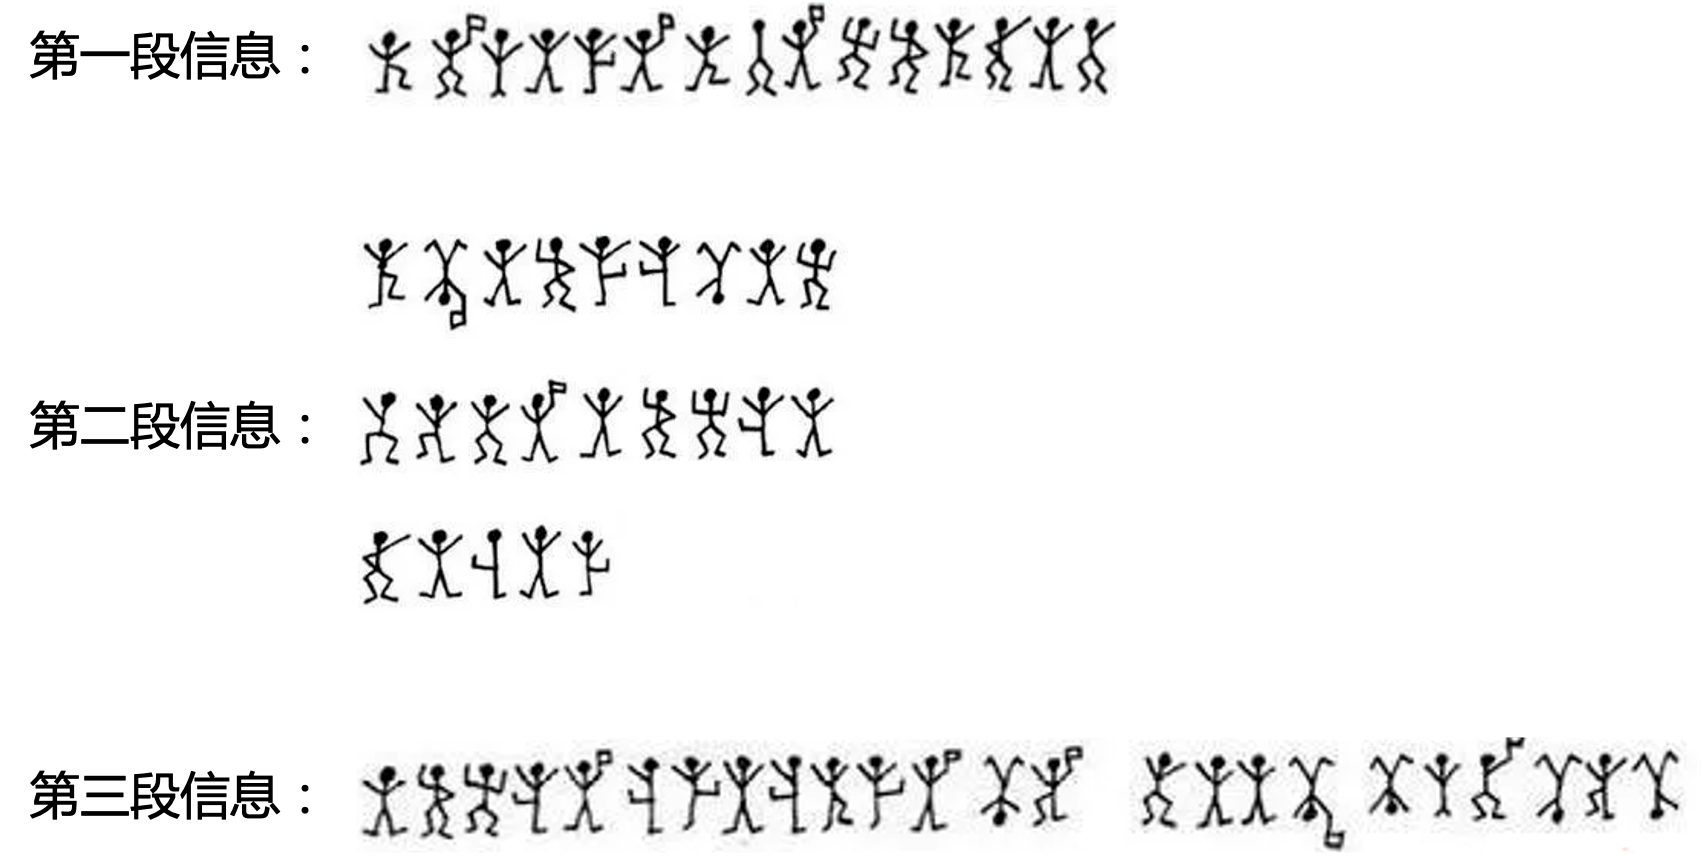
\includegraphics[width=0.75\linewidth]{image/Chap1DancingMen.png}
    \caption{跳舞小人密码}
\label{fig:chap01_dancing_men}
\end{figure}



可参考:https://zhuanlan.zhihu.com/p/372080601。
\end{example}

\subsection{确定概率的古典方法}
古典方法指的是在经验事实的基础上,对事件$A$的可能性进行逻辑分析后得出该事件的概率。其基本思想为所设计的随机现象只有有限个样本点,设为$n$个。每个样本点发生的可能性相等(称等可能性)。若事件$A$含有$k$个样本点,则是假$A$的概率为
    $$
    P(A) = \frac{k}{n}.
    $$
    
 \begin{example}
        投掷两枚硬币,如何求出现一正一反的概率?

        {\textbf{解}}:\quad 样本空间为$$\Omega= \{\text{(正,正),(正,反),(反,正),(反,反)} \}.$$于是,样本空间$\Omega$共有4个样本点。事件“出现一正一反”含有的样本点的个数为2。因此,所求的概率为$1/2$。
    \end{example}
古典方法是概率轮发展初期确定概率的常用方法,所得的概率又称为古典概率。在古典概率的计算中,经常使用排列组合工具。排列组合本质上都是计算“从$n$个元素中任取$r$个元素”的取法数量。组合不讲究取出元素间的次序,而排列讲究取出元素间的次序。常用的排列、组合有有以下四种:
 \begin{description}
        \item[排列]: 从$n$个不同的元素中任取$r(r\leq n)$个元素拍成一列(考虑元素先后出现次序)。这种排列数为
        $$P_n^r
        = n\times (n-1)\times \cdots \times (n-r+1) = \frac{n!}{(n-r)!}
        $$
        特别地,$r=n$时,称$P_n^n = n!$为全排列。
        \item[重复排列]:从$n$个不同元素中每次去处一个,放回后在取下一个,如此连续取$r$次所得的排列。这种重复排列数共有$n^r$个。注意:这里允许$r>n$。
        \item [组合]:从$n$个不同元素中任取$r(r\leq n)$个元素并成一组(不考虑元素间的先后次序)。这种组合数为$$
        C_n^r = \begin{pmatrix}n\\r\end{pmatrix}= \frac{n!}{r!(n-r)!}.
        $$
        特别地,(1) $0!=1$;(2)$\begin{pmatrix}n\\0\end{pmatrix} = 1$ ;(3) $\begin{pmatrix}n\\r\end{pmatrix}= \begin{pmatrix}n\\n-r\end{pmatrix}$。
        \item[重复组合]:从$n$个不同元素中每次取出一个,然后放回后再取下一个。如此连续取$r$次所得的组合。这种重复组合数为$\begin{pmatrix}n+r-1\\r\end{pmatrix} $。
            \end{description}
        \begin{example}
             从3个元素中抽2个元素,得到的重复组合数为多少?
        \end{example}
\begin{solution}
因为考虑到是重复组合,所以抽取出的元素可以重复,但是又不考虑元素之间的次序。所有的抽出的结果应为:11,12,13,22,23,33,共有6种。
\end{solution}
\begin{note}
    重复组合数的计算方式为:总共有$n$个元素,设为共有$n$个盒子,我们用$n+1$根棒子做间隔。如果第$i$个元素取到过一次,就标记一个“〇”。需要考虑重复组合数,除了不可动的头尾两根棒子之外,余下的棒子和盒子可以随意放置,于是,相当于在$n+r-1$个位置上任取$r$个放“〇”。因此,重复组合数为
    $$
    \begin{pmatrix}n+r-1\\r\end{pmatrix} = \begin{pmatrix}n+r-1\\ n-1\end{pmatrix}
    $$
\end{note}


\begin{example}[(不放回抽样)]
    一批产品共有9件,其中3件是不合格品,6件事合格品。从中不放回地随机抽出4件。试求事件$A_m=$“取出4件产品中有$m$个不合格品”的概率,$m=0,1,2,3$。
    \end{example}
    \begin{solution}
        \begin{eqnarray*}
    P(A_0) &=& \frac{C_6^4}{C_9^4} = \frac{15}{126} = \frac{5}{42} \\
     P(A_1) &=&   \frac{C_6^3\cdot C_3^1}{C_9^4} =  \frac{60}{126} = \frac{20}{42} \\
     P(A_2) &=&   \frac{C_6^2\cdot C_3^2}{C_9^4} =  \frac{45}{126} = \frac{15}{42} \\
      P(A_3) &=&   \frac{C_6^1\cdot C_3^3}{C_9^4} =  \frac{6}{126} = \frac{2}{42}
    \end{eqnarray*}
    \end{solution}
\begin{remark}
\begin{itemize}
    \item 这个问题中$m$可以看作一个{\textbf{随机变量}};
    \item $m$取$0,1,2,3$四种情况必有之一;
    \item $m$的概率分布(列)为\\
    \begin{table}[ht]
    \centering
    \begin{tabular}{c|cccc}
    \hline
    $m$ & $0$ & $1$ & $2$ & $3$\\
    \hline
    $P(A_m)$ & $\frac{5}{42}$ & $\frac{20}{42}$ &$\frac{15}{42}$ &$\frac{2}{42}$ \\
    \hline
    \end{tabular}
    \end{table}
    \end{itemize}
\end{remark}

    \begin{example}[(放回抽样)]
    从中有放回地随机抽出4件。试求事件$B_m=$“取出4件产品中有$m$个不合格品”的概率。
    \end{example}
    \begin{solution}
        \begin{eqnarray*}
    P(B_0) &=& \left(1-\frac{3}{9}\right)^4 = \left(\frac{2}{3}\right)^4 = \frac{16}{81} \\
     P(B_1) &=&   \frac{4\times 3^1 \times 6^3}{9^4} =  4\times \frac{3}{9} \times \left(\frac{6}{9}\right)^3 = \frac{32}{81} \\
     P(B_2) &=&    \frac{C_4^2\times 3^2 \times 6^2}{9^4} =  6\times \left(\frac{3}{9}\right)^1 \times \left(\frac{6}{9}\right)^2 = \frac{24}{81} \\
      P(B_3) &=&    \frac{C_4^3\times 3^3 \times 6^1}{9^4} =  4\times \left(\frac{3}{9}\right)^3 \times \left(\frac{6}{9}\right)^1 = \frac{8}{81} \\
      P(B_4) &=&     \left(\frac{3}{9}\right)^4 = \frac{1}{81} 
    \end{eqnarray*}
    \end{solution}

  \begin{example}[(盒子模型)]
    设有$n$个球,每个球都等可能地被放到$N$个不同盒子中的任一个。每个盒子所放球数不限。试求:\\
    \begin{itemize}
    \item 指定的$n(n\leq N)$个盒子中有一个球的概率$p_1$;
    \item 恰好有$n(n\leq N)$个盒子各有一个球的概率$p_2$;
    \end{itemize}
    \end{example}
    \begin{solution}
        \begin{itemize}
        \item $p_1 = \frac{n!}{N^n}$;
        \item $p_2 = \frac{C_N^n n!}{N^n} = \frac{P_N^n}{N^n} = \frac{N!}{N^n(N-n)!}$.
    \end{itemize}
    \end{solution}
    

 \begin{example}[(生日问题)]
    $n$个人的生日全不相同的概率$p_n$是多少?
    \end{example}
    \begin{remark}
        把$n$个人看成$n$个球,把一年365天看成$N=365$个盒子。因此,生日问题就转化为“恰好有$n$个盒子各有一球”的问题。
    \end{remark}


\subsection{确定概率的几何方法}
在几何方法中,一个随机现象的样本空间$\Omega$充满某个区域,其度量(长度、面积或提及)大小用$S_{\Omega}$表示。任意一点落在度量相同的子区域内(可能位置不同)是等可能的。若事件$A$为$\Omega$中某个子区域,且其度量大小可用$S_A$表示,则事件$A$的概率为
         $$
         P(A) = \frac{S_A}{S_{\Omega}}.
         $$
     
     \begin{example}[(会面问题)]
    甲乙两人约定下午6点到7点之间在某处会面,并约定先到者应等候另一个人20分钟,过时即可离去。求两人能会面的概率。
    \end{example}
\begin{solution}
设 $x,y$分别表示甲、乙到达约会地点的事件。根据题意,我们可以绘制一张图,如图\ref{fig:chap01_meeting}。图中蓝色区域是甲乙两人到达的时间的所有样本点,即样本空间$\Omega$,而甲乙两人能够会面的时间点在红色斜线的区域,记为$A$。于是计算途中对应的面积来得到概率,即
    \begin{eqnarray*}
        S_{\Omega} &=& 60^2 = 3600\\
        S_A &=& 3600 - 2 \times \frac{1}{2} \times 40^2= 2000\\
        P(A) &=& \frac{S_A}{S_{\Omega}} = \frac{2000}{3600} = \frac{5}{9}.
    \end{eqnarray*}
    \begin{figure}[ht]
        \centering
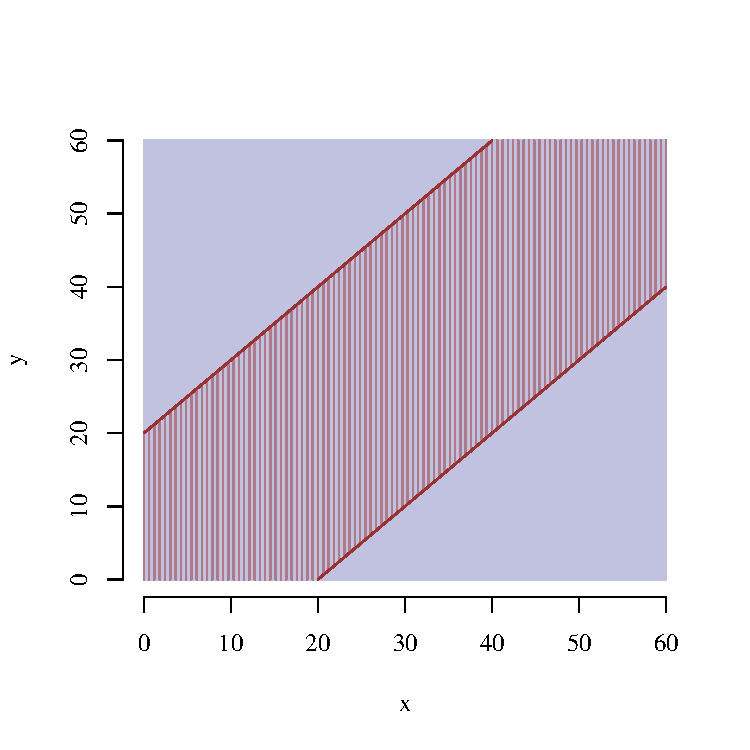
\includegraphics[width=0.6\linewidth]{image/Chap1Meeting.pdf}
        \caption{甲乙两人会面的几何概率示意图}
        \label{fig:chap01_meeting}
    \end{figure}
    \end{solution}
 \begin{example}[(蒲丰投针)]
    平面上画有间隔为$d(d>0)$的等距平行线,向平面任意投掷一枚长为$l$的针(l<d),求针与任一平行线相交的概率。
    \end{example}
    \begin{solution}
        设 $x$ 为针的中点与最近一条平行线的距离,$\phi$ 为针与此直线间的夹角。于是,$x$和$\phi$满足
    $$
    0\leq x\leq \frac{d}{2}, \quad 0\leq \phi \leq \pi.
    $$
    所以,$$
    S_{\Omega} = \frac{\pi d}{2}.
    $$
    而针与平行线相交,$\Leftrightarrow x\leq \frac{l}{2}\sin\phi$。所以,
    $$
    S_A = \int_0^{\pi} \frac{l}{2} \sin \phi \text{d} \phi  = \frac{l}{2} \left(-\cos \phi |_0^{\pi}\right) = \frac{l}{2}\times 2 = l.
    $$
    因此,所求的概率为
    $$
    P(A) = \frac{S_A}{S_{\Omega}} = \frac{l}{\frac{\pi d}{2}} = \frac{2l}{\pi d}.
    $$
    \end{solution}
\begin{remark}
  \begin{itemize}
    \item 当$l$与$d$已知时,$P(A)$可计算;
    \item 如果已知$P(A)$,那么可以近似$\pi$。(蒲丰投针实验是近似$\pi$值的有名实验)
    \item 只要设计一个随机试验,使得一个事件的概率与某个未知数有关,然后重复试验,以频率估计概率,即可求出未知数的近似值。
    \item 这个方法称为\textbf{随机模拟法}。
\end{itemize}  
\end{remark}


\section{概率的性质}
\subsection{有限可加性}
\begin{lemma}\label{lem:chap01_impossible_set}
如果事件$\emptyset$是不可能事件,则$P(\emptyset)=0$。
\end{lemma}
\begin{proof}
    令$A_1 = \Omega$,而$A_i = \emptyset,i=2,3,\cdots$。当$i\neq j$,有$A_i A_j = \emptyset$,于是所构造的$A_1,A_2,\cdots,A_n,\cdots$是一列互不相容的随机事件。根据概率的公理化定义中可列可加性,我们有
    \begin{eqnarray*}
        1 = P(\Omega) &=& P(\cup_{n=1}^\infty A_n)\\
        &=& \sum_{n=1}^\infty P(A_n)\\
        &=& P(\Omega) + \sum_{n=2}^\infty P(\emptyset)\\
        &= & 1 + \sum_{n=2}^\infty P(\emptyset)
    \end{eqnarray*}
    并根据概率的公理化定义中非负性有
    $$
    P(\emptyset) = 0.
    $$
\end{proof}
\begin{theorem}[有限可加性]\label{thm:chap01_finite_additivity}
若有限个事件$A_{1} ,A_{2} ,\dots ,A_{n} $ 互不相容,则有$$P\left(\bigcup_{i=1}^{n}A_{i}  \right)=\sum_{i=1}^{n } P(A_{i} )$$。
\end{theorem}
\begin{proof}
令$A_{n+1} = A_{n+2} = \cdots = \emptyset$。根据
概率的公理化定义中可列可加性,我们有
\begin{eqnarray*}
    P(\cup_{k=1}^n A_k) &=& P(\cup_{n=1}^\infty A_n)\\
    &=& \sum_{n=1}^\infty P(A_n)\\
    &=& \sum_{k=1}^n P(A_k) + \sum_{k=n+1}^\infty P(A_k)\\
    &=& \sum_{k=1}^n P(A_k)
\end{eqnarray*}
其中,最后一个等式成立是因为对于$k\geq n+1,A_k = \emptyset$,所以根据引理\ref{lem:chap01_impossible_set},$P(A_k)=0$。
\end{proof}
\begin{corollary}
对任一事件A,有$P(\overline{A} )=1-P(A)$。
\end{corollary}
\subsection{概率的单调性}
\begin{lemma}\label{lem:chap01_probability_difference}
若$A\supset B$ ,则$P(A-B)=P(A)-P(B)$。
\end{lemma}
\begin{proof}
    当$A\supset B$时,$A = B \cup (A-B)$,而且$B$与$A-B$是互不相容的。根据定理\ref{thm:chap01_finite_additivity}有,
    $$
    P(A) = P(B) + P(A-B),
    $$
    所以,
    $$
    P(A-B) = P(A) - P(B).
    $$
\end{proof}
\begin{theorem}[概率的单调性]\label{thm:chap01_probability_monotone}
    若$A\supset B$ ,则$P(A)\geq P(B)$。
\end{theorem}
\begin{proof}
根据引理\ref{lem:chap01_probability_difference},$$P(A-B) = P(A) - P(B).$$
因为概率的非负性,即$P(A-B) \geq 0$,所以,
$$
P(A) \geq P(B).
$$
\end{proof}

\subsection{概率的半可加性}
\begin{lemma}\label{lem:chap01_probability_difference_2}
    $\forall A,B$,有$P(A-B)=P(A)-P(AB)$。
\end{lemma}
\begin{proof}
    因为$A = (A-B) \cup AB$,而且这两个事件均是互不相容的。根据定理\ref{thm:chap01_probability_monotone},有
    $$
    P(A) = P(A-B) + P(AB).
    $$
    于是,
    $$
    P(A-B) = P(A) - P(AB).
    $$
\end{proof}
\begin{remark}
    引理\ref{lem:chap01_probability_difference_2}与引理\ref{lem:chap01_probability_difference}的结论是类似的。注意到,当$A\supset B$,$AB=B$。因此,引理\ref{lem:chap01_probability_difference}是引理\ref{lem:chap01_probability_difference_2}的一种特例。
\end{remark}
对任意两个事件$A,B$,有$$P(A\cup B)=P(A)+P(B)-P(AB)$$。

\begin{lemma}\label{lem:chap01_probability_addition}
    对任意两个事件$A,B$,有$$P(A\cup B)\leq P(A)+P(B).$$
\end{lemma}
\begin{proof}
    因为 $A\cup B = (A-B) \cup (B-A) \cup AB$,而且这三个事件均是互不相容的。根据定理\ref{thm:chap01_finite_additivity},有
    \begin{eqnarray*}
        P(A\cup B) &=& P(A-B) + P(B-A) + P(AB)\\
        &=& P(A-B) + P(AB) + P(B-A) + P(AB) - P(AB)\\
        &=& P(A) + P(B) - P(AB),
    \end{eqnarray*}
    其中最后一个等式成立是因为引理\ref{lem:chap01_probability_difference_2}。因此定理得证。
\end{proof}
\begin{theorem}[概率的半可加性]
    对任意两个事件$A,B$,有$$P(A\cup B)\leq P(A)+P(B).$$
\end{theorem}
 \begin{proof}
 根据引理\ref{lem:chap01_probability_addition},有
 $$
 P(A\cup B) = P(A) + P(B) - P(AB).
$$
又因为概率公理化定义中的非负性,有
$$P(A\cup B)\leq P(A)+P(B).$$
 \end{proof}
 \begin{corollary}\label{cor:chap01_probability_half_additivity_n}
     对任意$n$个事件$A_{1} ,A_{2} ,\dots ,A_{n} $ ,有$$P(\bigcup_{i=1}^{n}A_{i}  )\le \sum_{i=1}^{n } P(A_{i} ).$$
 \end{corollary}
  \begin{remark}
      推论\ref{cor:chap01_probability_half_additivity_n}也是统计学和机器学习在理论推导时的一个重要技巧,可以通过缩放来得到误差的上界。
  \end{remark}
\subsection{概率的连续性(选修内容)}
 \begin{definition}[极限事件] \label{def:limit event} 
  \begin{enumerate}
      \item 对$\mathcal{F}$中任一单调不减的事件序列$F_{1} \subset F_{2}\subset \cdots \subset F_{n}\subset \cdots $,称可列并且 $\bigcup_{n=1}^{\infty } F_{n}$为 $\{F_{n}\}$的极限事件记为$$\lim_{n \to \infty} F_{n} =\bigcup_{n=1}^{\infty } F_{n}. $$
      \item 对$\mathcal{F}$中任一单调不增的事件序列$E_{1} \supset E_{2}\supset \cdots \supset E_{n}\supset \cdots $,称可列并且 $\bigcap_{n=1}^{\infty } E_{n}$为 $\{E_{n}\}$的极限事件记为$$\lim_{n \to \infty} E_{n} =\bigcap_{n=1}^{\infty } E_{n}. $$
  \end{enumerate}
  \end{definition}
  
    \begin{definition}[上、下连续] \label{def:continuity} 
    对$\mathcal{F}$上的一个概率$P$,\\
    (1)若其对 $\mathcal{F}$中任一单调不减的事件序列 $\{F_{n}\}$均成立,$$\lim_{n \to \infty} P(F_{n} )=P(\lim_{n \to \infty}F_{n}  )$$
    则称概率$P$是下连续的。\\
    (2)若其对 $\mathcal{F}$中任一单调不增的事件序列 $\{E_{n}\}$均成立,$$\lim_{n \to \infty} P(E_{n} )=P(\lim_{n \to \infty}E_{n}  )$$
    则称概率$P$是上连续的。
  \end{definition}

\begin{theorem}[概率的连续性]\label{thm:chap01_probabilty_continuity}
若$P$为事件域$\mathcal{F}$上的概率,则$P$既是下连续的又是上连续的。
\end{theorem}

\begin{proof}
先证$P$的下连续性。\\
设 $\left \{ F_{n}  \right \} $是 $\mathcal{F}$中一个单调不减的事件序列,即$$\lim_{n \to \infty} F_{n} =\bigcup_{n=1}^{\infty } F_{n}$$
若定义 $F_{0} =\phi $,则$$\bigcup_{i=1}^{\infty } F_{i}=\bigcup_{i=1}^{\infty }(F_{i}-F_{i-1})$$
由于$F_{i-1} \subset F_{i}$ ,显然 $\left (  F_{i}-F_{i-1}  \right ) $两两不相容,再由可列可加性得
\begin{equation}
  \begin{aligned}
   P(\bigcup_{i=1}^{\infty }F_{i}  )
   &=P(\bigcup_{i=1}^{\infty }(F_{i}-F_{i-1})) \\
   &=\sum_{i=1}^{\infty } P(F_{i}-F_{i-1}) \\
   &=\lim_{n\to \infty} \sum_{i=1}^{n } P(F_{i}-F_{i-1})\\
   &=\lim_{n\to \infty} P( \bigcup_{i=1}^{n}  (F_{i}-F_{i-1}  ) )\\
   &=\lim_{n\to \infty} P( F_{n} )\\
  \end{aligned}
\end{equation}
所以,概率$P$的下连续性由此得证。\\
再证概率$P$的上连续性。\\
设 $\left \{ E_{n}  \right \} $是单调不增的事件序列,则$\left \{ \overline{E_{n} }  \right \} $为单调不减的事件序列,由概率的下连续性可得
\begin{equation}
  \begin{aligned}
   1-\lim_{n\to \infty} P(E_{n} )
   &=\lim_{n\to \infty } (1-P(E_{n}))\\
   &=\lim_{n\to \infty } P(\overline{E_{n} } )\\
   &=P(\bigcup_{n=1}^{\infty } \overline{E_{n} } )\\
   &=P(\overline{\bigcap_{n=1}^{\infty } E_{n} }  )\\
   &=1-P(\bigcap_{n=1}^{\infty } E_{n}   )\\
  \end{aligned}
\end{equation}
因此,$$\lim_{n \to \infty} P(E_{n} )=P(\bigcap_{n=1}^{\infty } E_{n} )=P(\lim_{n \to \infty}E_{n} )$$
这就证明了概率$P$的上连续性。\\
\end{proof}

\begin{remark}
    概率的公理化定义中,可以将可列可加性换成有限可加性和下连续性.
\end{remark}

\section{习题}
    \begin{enumerate}
        \item 某城市中共发行3种报纸$A,B,C$.在这城市的居民中有$45\%$订阅$A$报、$35\%$订阅$B$报、$30\%$订阅$C$报、$10\%$同时订阅$A$报$B$报、$8\%$同时订阅$A$报$C$报、$5\%$同时订阅$B$报$C$报、$3\%$同时订阅$A,B,C$报.求以下事件的概率:
        \begin{enumerate}
            \item 只订阅$A$报的;
            \item 只订阅一种报纸的;
            \item 至少订阅一种报纸的;
            \item 不订阅任何一种报纸的。
        \end{enumerate}
\item 证明:
\begin{enumerate}
    \item $P(AB) \geq P(A)+P(B)-1$;
    \item 请把(1)中的结果推广至$n$个随机事件的结果,即
$P(A_1 A_2\cdots A_n) \geq P(A_1)+P(A_2)+\cdots+P(A_n)-(n-1)$。
\end{enumerate}


\item 反复掷四面骰子,直到第一次(如果有的话)得到偶数面。这个实验的样本空间是多少?

\item 在8*8的棋盘上,八个“车”被放置在不同的方格中,放的所有可能的位置都是等概率的。找出所有“车”彼此安全的概率,即没有包含超过一个“车”的行或列。

\item 一个箱子里有$n$个球,其中$m$个是红色的。
\begin{enumerate}
    \item 我们随机选择$k$个球,不放回(即在下一次选择之前,选定的球不会放回箱子里)。那么挑选出来$k$个球中$i$个是红球的概率是多少?
    \item 我们随机选择$k$个球,有放回(即在下一次选择之前,选定的球会放回箱子里)。那么挑选出来$k$个球中$i$个是红球的概率是多少?
\end{enumerate}

\item 口袋中有10个球,分别标有号码从1到10,现从口袋中不放回地任取其中4个,记下取出的球的号码,试求:
\begin{enumerate}
\item 4个球中最小号码为5的概率;
\item 4个球中最大号码为5的概率。
\end{enumerate}

\item  把$n$个“0”和$n$个“1”随机地排列,求没有两个“1”连在一起的概率。
    \end{enumerate}
% \begin{exercise}
% \end{exercise}


